
\section*{Problema P8.10}

\renewcommand*\thesection{8.10}
\numberwithin{equation}{section}

\begin{center}
    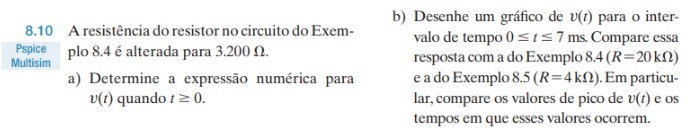
\includegraphics[scale=1.0]{P8.10.jpg}
\end{center}

\subsection*{(a)}

O circuito do Exemplo 8.4 é um circuito RLC paralelo, com equação característica já conhecida:

\begin{equation}\label{eq:8.10.1}
    s^2 + \frac{s}{RC} + \frac{1}{LC} = 0
\end{equation}

Substituindo com os valores do enunciado,

\[ s = \frac{-(2500) \pm \sqrt{(2500)^2 - 4(1)(1 \cdot 10^6)}}{2(1)} \]

\[ s_1 = -500 \un{rad/s} \quad , \quad s_2 = -2000 \un{rad/s} \]

Agora analisamos as condições iniciais do circuito. Temos

\begin{equation}\label{eq:8.10.2}
    v(0) = 0 \un{V}
\end{equation}

Para a condição de inicial de $\diff{v(0)}{t}$, aplicamos análise nodal no nó superior do circuito em $t=0$, obtendo

\[ i_c(0) + i_L(0) + i_R = 0  \]

\[ i_c(0) + -12.25 \un{mA} + \frac{v(0)}{20\un{k$\Omega$}} = 0  \]

\[ i_c(0) = 12.25 \un{mA}  \]

Note que

\[ i_c = C\diff{v}{t} \logo \diff{v(0)}{t} = \frac{i_c(0)}{C} \]

Assim, subsituindo o valor de $i_c(0)$ encontrado, temos a segunda condição inicial da EDO dada por

\begin{equation}\label{eq:8.10.3}
    \diff{v(0)}{t} = 98000 \un{V/s}
\end{equation}

Além disso, sabemos que a solução da EDO é da forma

\[ v(t) = Ae^{st}  \]

Com as duas raízes encontradas $s_1$ e $s_2$, temos que a solução geral é dada pela combinação linear

\begin{equation}\label{eq:8.10.4}
    v(t) = v_1(t) + v_2(t)
\end{equation}

Onde $v_1(t)$ e $v_2(t)$ são duas possíveis soluções para $v(t)$ dadas por  

\[ \begin{cases}
        v_1(t) = A_1e^{s_1t}  & \\
        \noalign{\vskip9pt}
        v_2(t) = A_2e^{s_2t}
    \end{cases}
\]

Diferenciando \eqref{eq:8.10.4} com respeito a $t$, temos duas equações

\[ \begin{cases}
        v(t) = A_1e^{s_1t} + A_2e^{s_2t} & \\
        \noalign{\vskip9pt}
        \diff{v(t)}{t} = A_1s_1e^{s_1t} + A_2s_2e^{s_2t}
    \end{cases}
\]

Em $t=0$, temos as condições iniciais já conhecidas em \eqref{eq:8.10.2} em \eqref{eq:8.10.3}

\[ \begin{cases}
        v(0) = A_1e^{s_10} + A_2e^{s_20} & \\
        \noalign{\vskip9pt}
        \diff{v(0)}{t} = A_1s_1e^{s_10} + A_2s_2e^{s_20}
    \end{cases}
    \logo
    \begin{cases}
        A_1 + A_2 = 0 \un{V} & \\
        \noalign{\vskip9pt}
        A_1s_1 + A_2s_2 = 98000 \un{V/s}
    \end{cases}
    \logo
    \begin{cases}
        A_1 =  65.33 & \\
        \noalign{\vskip9pt}
        A_2 = -65.33
    \end{cases}
\]

Conhecidos coeficientes $A_1$ e $A_2$, bem como as raízes $s_1$ e $s_2$, temos a solução geral $v(t)$ dada por  \eqref{eq:8.10.4}

\[ \boxed{v(t) = 65.33\left[e^{-500t} - e^{-2000t}\right] \un{V} \, , \, t \geq 0 }  \]

\subsection*{(b)}

Temos três funções para $v(t)$:

\[ \begin{cases}
        v(t) = 65.33\left[e^{-500t} - e^{-2000t}\right] \un{V} \, , \, t \geq 0  & \textrm{Resposta superamortecida} \\
        \noalign{\vskip9pt}
        v(t) = 98.000te^{-1.000t} \un{V} \, , \, t \geq 0 & \textrm{Resposta criticamente amortecida} \\
        \noalign{\vskip9pt}
        v(t) = 100e^{-200t} sen (979.80t) \un{V} \, , \, t \geq 0 & \textrm{Resposta subamortecida} \\
    \end{cases}
\]

Usando a ferramenta online Desmos, temos os três gráficos das três funções abaixo. A curva vermelha é a subamortecida, a
preta é a criticamente amortecida e a curva verde é a resposta superamortecida. \\
A resposta subamortecida apresenta o maior valor de pico da tensão, mas é a que gasta mais tempo para ele ocorrer. 
Já a resposta superamortecida possui o menor valor de pico, mas é o que chega mais rápido nesse pico.

\begin{center}
    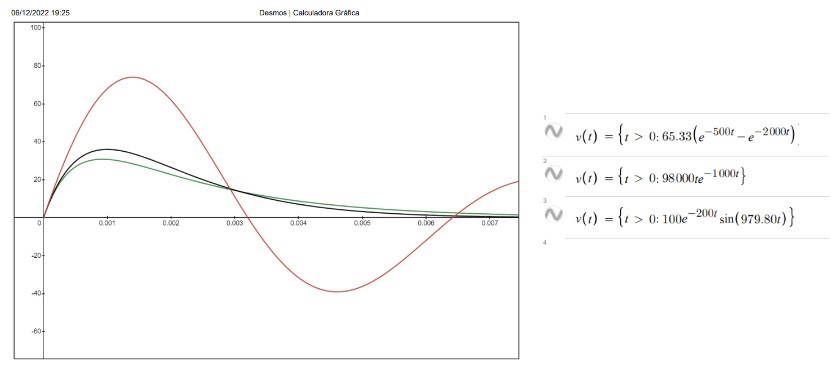
\includegraphics[scale=1.0]{P8.10-Item(b).jpg}
\end{center}






